\documentclass[a4paper]{article}

%%%%%%%% CREATE DOCUMENT STRUCTURE %%%%%%%%
%% Language and font encodings
\usepackage[english]{babel}
\usepackage[utf8x]{inputenc}
\usepackage[T1]{fontenc}
%\usepackage{subfig}

%% Sets page size and margins
\usepackage[a4paper,top=3cm,bottom=2cm,left=2cm,right=2cm,marginparwidth=1.75cm]{geometry}

%% Useful packages
\usepackage{amsmath}
\usepackage{amssymb}
\usepackage{graphicx}
\usepackage[colorinlistoftodos]{todonotes}
\usepackage[colorlinks=true, allcolors=blue]{hyperref}
\usepackage{caption}
\usepackage{subcaption}
\usepackage{sectsty}
\usepackage{apacite}
\usepackage{float}
\usepackage{titling} 
\usepackage{blindtext}
\usepackage[square,sort,comma,numbers]{natbib}
\usepackage[colorinlistoftodos]{todonotes}
\usepackage{xcolor}
\definecolor{darkgreen}{rgb}{0.0, 0.4, 0.0}

%%%%%%%% DOCUMENT %%%%%%%%
\begin{document}

%%%% Title Page
\begin{titlepage}

\newcommand{\HRule}{\rule{\linewidth}{0.5mm}} 							% horizontal line and its thickness
\center 
 

\includegraphics[width=0.2\textwidth]{images/download.png}\\[1cm] 	
% University logo
% University
\textsc{\LARGE Bangladesh University of Engineering \& Technology}\\[1cm]

% Document info
\textsc{\underline{\textbf{\Large 1805004}}}\\[1cm]
\textsc{\Large COURSE}\\[0.2cm]
\textsc{\large CSE 204}\\[0.5cm] 		
% Document info
\textsc{\large Data Structures and Algorithms I Sessional}\\[1.5cm] 	
% Course Code
\HRule \\[0.8cm]
{ \huge \bfseries Report On:}\\[0.7cm]	
\textsc{\large Offline 8 Complexity Analysis}\\[1cm] 
{ \huge \bfseries Topic:}\\[0.7cm]	
\textsc{\large Divide \& Conquer}\\[1cm] 
% Assignment
\HRule \\[1.5cm]
\large
\textsc{\emph\large{Author:}}\\
Syed Jarullah Hisham\\
\textbf{Roll: 1805004}\\
CSE'18 Section A1\\[1.5cm]		

{\large \today}\\[5cm]
% Author info
\vfill 
\end{titlepage}


%%Your abstract.
%%\end{abstract}

%%%% SECTIONS
%% Section 1
\large
\section*{\centerline{Time Complexity Analysis}}
Divide and conquer approach was used to correctly find the second nearest pair of houses. This approach takes O(nlogn) time to execute. The step by step time complexity with its algorithm is described below:\\\\
\centerline{\textbf{\underline{Preprocess}}}\\\\
\textbf{\underline{Step 1:}}\\\\
        Firstly, two array were created and sorted according to Y and X-coordinates. 
        We will call these arrays as X-array and Y-array in the upcoming discussions. By default, java uses merge sort algorithm to sort user defined objects’ array. So, this step requires O(nlogn) time. Other operations like initialiing or copy array all take less time i.e O(n) time. \textbf{So, overall the time complexity of this step is O(nlogn)}.\\\\
\textbf{\underline{Step 2:}}\\\\
       If total number of points are 3, then brute force algorithm is used which takes constant amount of time, \textbf{so this step requires O(1) time}.\\
       
         Next, nearest pair of point algorithm is called.\\\\\\
\textbf{\centerline{\underline{Nearest Pair of Point Algorithm}}}\\\\
\textbf{\underline{Step 3:}}\\\\
\textbf{\underline{Divide \& Conquer:}}\\\\
        It is one of the most important step of this algorithm. The points which were sorted by X-coordinates are divided into two equal halves (left part and right part) and recursively call nearest pair of point algorithm to find the value of delta (the lowest distance of two points in a particular subarray). As we divide original array into two subarrays and recursively call the algorithm, this step is called the divide \& conquer step of this algorithm. This step does two things. One, finding value of delta and other is recursively sort the Y-array. If we T(n) be the running time of this whole step then the divide step requires T(n/2) time. And after calling these methods, we call merge method to ensure that the Y-array are correctly sorted according to Y-coordinates. This merge method requires O(n) time.\\\\
        So, by observing the step 2 \& 3, we can figure out a simple recursive equation. \\\\
Let, T(n) is the running time of this step. 

\[
  T(n) =
  \begin{cases}
                                   O(1) & \text{if $n=3$} \\
  2 T(n/2) + O(n) & \text{if $n>3$}
  \end{cases}
\]
Now, using the master theorem, we can prove that T(n) = O(nlogn).
\textbf{So, the divide \& conquer step requires O(nlogn) time}.\\\\\\
\textbf{\underline{Step 4:}}\\\\
\textbf{\underline{Merge Step:}}\\\\
        This is the trickiest and most important part of the analysis. In this step, firstly, based on the value of delta, we will create an array of strip covering the region with all points which are at most delta distance away from the middle line dividing the two sets. \textbf{This strip creation takes O(n) time}.\\\\
        Next, the smallest distance in strip is determined. For this, we use nested loop to find the minimum distance. So, at first look, it is seen that finding smallest distance requires O(${n}^2$) time. \textbf{But actually, it is O(n)}. It can be proved geometrically that for every point in strip, we only need to check at most 7 points after it. \\\\
        We can prove it by the following approach: \\\\
\textbf{Theorem}:  Let, any point in the box $P_k$ and any pair of point is $Y_i$ and $Y_j$.  We have to prove that there are at most 7 other points such that $Y_i$ – $Y_j$ <= delta.\\\\
\textbf{Proof}:
\begin{figure}[H]
\center
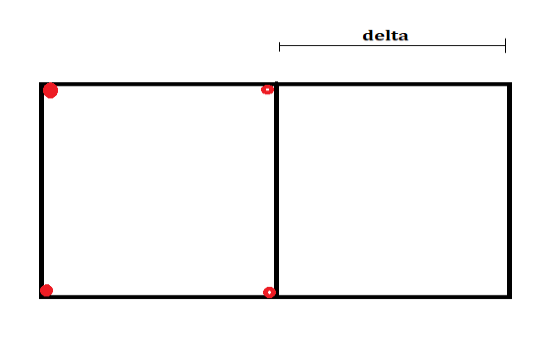
\includegraphics{images/box.png}
\caption{delta covered squared area}
\end{figure}
\begin{itemize}
  \item In the figure, left and right square have equal area of delta * delta.
  \item So, all points Pk must lie in anyone of left and right sides.
  \item Having delta at each side, we can say that all points have distance <=        delta from others.
  \item As we have two squares, and each having 4 points at the corners; we get       total 8  points. If Pk is one point, then there are 7 other points.
\end{itemize}
$\therefore$ There are at most 7 other points in the range of delta other than the point itself. So, we have to check at most 7 points to find the nearest distance.\\\\
So, the total loop operation is at most 7*n times. As 7 is a constant, it takes constant time to execute the inner loop. $\therefore$ \textbf{total required runtime for merge step is O(n)}.
\textbf{\centerline{\underline{Second Nearest Pair of Points}}}\\\\
\textbf{\underline{Step 5:}}\\\\
          This step simply applies nearest pair finder algorithm twice ignoring one of the nearest pair each time that we found in previous step. Finally, find the second nearest pair comparing the results of this two. \textbf{So, this step requires O(nlogn) time}.\\\\
\fbox{
\centerline{
\parbox{\textwidth}{
\begin{center}
 So, total cost of the whole algorithm is:\\
\textbf{
Sorting + Nearest Pair of points + Second nearest pair of points\\
= O(nlogn) + O(nlogn) + O(nlogn)\\
= O(nlogn)
}
\end{center}
}
}
}\\\\\\
\section*{\centerline{Time Complexity Using Code Snippet}}
\centerline{Here is a code snippet showing a summary of time complexity of the whole algorithm}
\hfill \break
\begin{figure}[H]
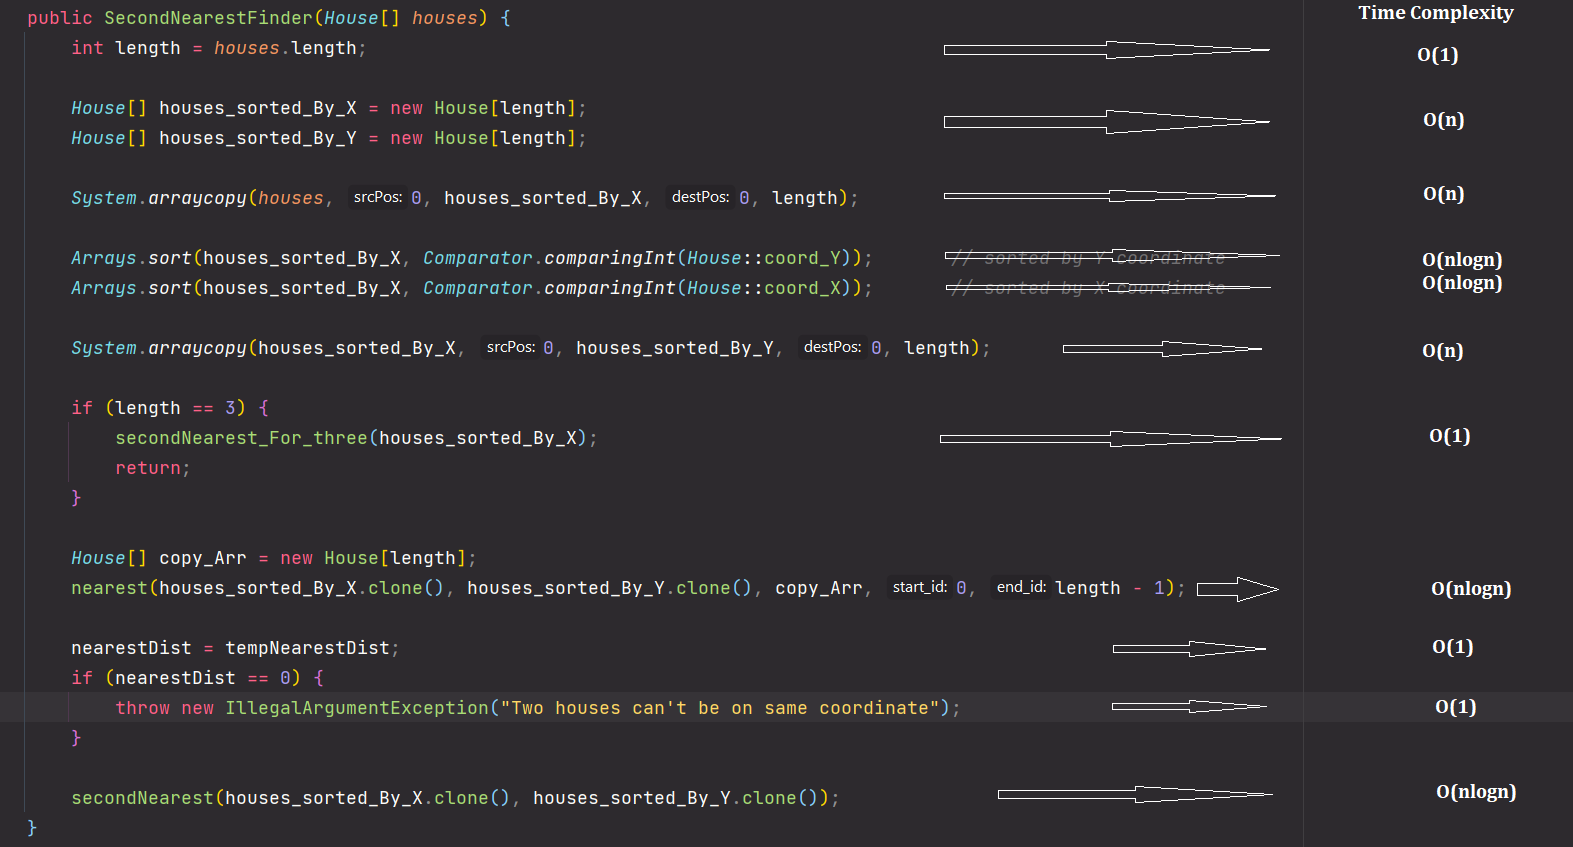
\includegraphics[width=1.05\textwidth, height=10cm]{images/Time Analysis_1.png}
\end{figure}

\end{document}